\documentclass[12pt]{article}
        \makeatletter
        \def\input@path{{../../}}
        \makeatother
        \usepackage{sbc-template}
        \makeatletter
        \renewcommand{\inst}[1]{}
        \makeatother
        \usepackage{graphicx,url}
        \usepackage[utf8]{inputenc}
        \usepackage[T1]{fontenc}
        \usepackage[brazil]{babel}
        \usepackage{longtable,booktabs,array}
        \usepackage{amsmath,amssymb}
        \providecommand{\tightlist}{%%
          \setlength{\itemsep}{0pt}\setlength{\parskip}{0pt}}
        \sloppy
        \title{Quantum Reservoir Computing para previsao de demanda: um estudo didatico com o Favorita}
        \author{}
        \address{}
        \begin{document}

        \maketitle

        \begin{resumo}
        Este artigo fecha a serie com um estudo completo e didatico de Quantum Reservoir Computing (QRC) aplicado ao recorte do Favorita adotado desde o primeiro capitulo. O texto unifica tudo o que foi construido anteriormente: problema de negocio, protocolo experimental, benchmark justo, intuicao de reservatorio e ponte conceitual para o quantico. Em seguida, apresenta o pipeline do QRC implementado com Qiskit, compara as configuracoes \texttt{14x7} e \texttt{8x5}, discute a funcao objetivo usada no tuning e posiciona os resultados do QRC ao lado de \texttt{ETS}, \texttt{XGBoost} e \texttt{RC}. O resultado final e instrutivo: o QRC funciona de ponta a ponta, \texttt{14x7} e a melhor configuracao por desempenho puro, \texttt{8x5} e o melhor compromisso pela funcao objetivo, mas as tecnicas classicas seguem superiores neste recorte.
        \end{resumo}

        \subsection{1. O que o leitor vai aprender}\label{1-o-que-o-leitor-vai-aprender}

Ao final deste artigo, voce sera capaz de:

\begin{enumerate}
\def\labelenumi{\arabic{enumi}.}
\tightlist
\item
  descrever o pipeline completo de QRC do projeto;
\item
  executar o modelo com Qiskit no recorte do Favorita;
\item
  interpretar por que \texttt{14x7} e \texttt{8x5} coexistem como candidatos fortes;
\item
  comparar o QRC com RC e modelos classicos no mesmo protocolo;
\item
  concluir o que a serie inteira ensina sobre a rota ate QRC.
\end{enumerate}

\subsection{2. O recorte experimental herdado da serie}\label{2-o-recorte-experimental-herdado-da-serie}

O estudo final nao muda o problema para favorecer o QRC. Ele preserva:

\begin{itemize}
\tightlist
\item
  \texttt{store\_nbr\ =\ 1}
\item
  \texttt{family\ =\ BEVERAGES}
\item
  frequencia diaria
\item
  ultimos \texttt{90} dias como teste
\end{itemize}

Isso garante continuidade didatica e comparabilidade cientifica.

\subsection{3. Pipeline de QRC usado no projeto}\label{3-pipeline-de-qrc-usado-no-projeto}

\subsubsection{3.1 Entrada}\label{31-entrada}

O QRC usa um vetor de entrada classico reduzido:

\[
u_t =
\begin{bmatrix}
\widetilde{y}_{t-1} &
\widetilde{p}_t &
\sin(2\pi \, \mathrm{dow}_t / 7) &
\cos(2\pi \, \mathrm{dow}_t / 7)
\end{bmatrix}^\top.
\]

Essa reducao aparece em \texttt{\_quantum\_input\_vector()}, que seleciona os quatro primeiros componentes do vetor sequencial classico.

\subsubsection{3.2 Dinamica quantica}\label{32-dinamica-quantica}

Para cada passo da janela, o circuito aplica rotacoes \texttt{RX} e \texttt{RY} em todos os qubits e um anel de emaranhamento \texttt{CZ} + \texttt{RZ}. Se chamarmos o operador de um passo de \(U(u_t)\), a representacao da janela fica

\[
|\psi_t\rangle = U(u_t) U(u_{t-1}) \cdots U(u_{t-w+1}) |0 \cdots 0\rangle.
\]

\subsubsection{3.3 Observaveis}\label{33-observaveis}

As features quanticas sao expectativas:

\[
z_t^{(j)} = \langle \psi_t | O_j | \psi_t \rangle.
\]

O projeto usa observaveis \texttt{Z}, \texttt{X} e \texttt{ZZ}, totalizando \texttt{3q} componentes para \texttt{q} qubits.

\subsubsection{3.4 Readout}\label{34-readout}

O readout final continua sendo simples:

\[
\hat{y}_t = W_{out} [1; u_t; z_t],
\]

com treinamento Ridge:

\[
W_{out}^* = \arg\min_{W_{out}} \|Y - \Phi W_{out}\|_2^2 + \lambda \|W_{out}\|_2^2.
\]

Em outras palavras, o QRC do projeto herda a filosofia central de RC: dinamica rica, readout simples.

\subsection{4. Implementacao passo-a-passo}\label{4-implementacao-passo-a-passo}

O leitor pode percorrer a implementacao nesta ordem.

\subsubsection{4.1 Passo 1: definir a configuracao}\label{41-passo-1-definir-a-configuracao}

\begin{verbatim}
@dataclass(frozen=True)
class QRCConfig:
    n_qubits: int = 14
    window: int = 7
    input_scale: float = 1.2
    ridge_alpha: float = 1e-1
    seed: int = 7
\end{verbatim}

\subsubsection{4.2 Passo 2: construir o circuito por passo}\label{42-passo-2-construir-o-circuito-por-passo}

O codigo central esta em \texttt{\_step\_circuit()} e usa \texttt{QuantumCircuit} do Qiskit.

\subsubsection{4.3 Passo 3: acumular a janela quantica}\label{43-passo-3-acumular-a-janela-quantica}

\texttt{features\_from\_window()} compoe sucessivos passos do circuito antes de criar o \texttt{Statevector}.

\subsubsection{4.4 Passo 4: medir observaveis}\label{44-passo-4-medir-observaveis}

O metodo \texttt{\_build\_observables()} cria as listas de operadores \texttt{Z}, \texttt{X} e \texttt{ZZ}.

\subsubsection{4.5 Passo 5: ajustar o readout e prever}\label{45-passo-5-ajustar-o-readout-e-prever}

\texttt{fit\_qrc\_readout()} treina o Ridge e \texttt{forecast\_qrc()} faz previsao recursiva no bloco de teste.

Para executar:

\begin{verbatim}
python code/qrc/run.py
pytest code/qrc/test_model.py
pytest code/qrc/test_objective.py
\end{verbatim}

\subsection{5. Configuracao experimental}\label{5-configuracao-experimental}

O tuning anterior deixou duas configuracoes principais:

\begin{itemize}
\tightlist
\item
  melhor configuracao por rank medio multi-metrica: \texttt{14x7}
\item
  melhor configuracao pela funcao objetivo escalar: \texttt{8x5}
\end{itemize}

O artigo final preserva as duas porque elas respondem a perguntas diferentes:

\begin{itemize}
\tightlist
\item
  "qual performa melhor nas metricas?" -\textgreater{} \texttt{14x7}
\item
  "qual equilibra melhor desempenho e complexidade?" -\textgreater{} \texttt{8x5}
\end{itemize}

\subsection{6. Resultados do QRC}\label{6-resultados-do-qrc}

A comparacao direta entre as duas configuracoes ficou assim:

\begin{longtable}[]{@{}lllll@{}}
\toprule\noalign{}
Modelo & MAE & RMSE & WAPE & sMAPE \\
\midrule\noalign{}
\endhead
\bottomrule\noalign{}
\endlastfoot
QRC14x7 & 441.286 & 525.325 & 0.2038 & 0.2269 \\
QRC8x5 & 455.833 & 526.949 & 0.2105 & 0.2342 \\
\end{longtable}

\pandocbounded{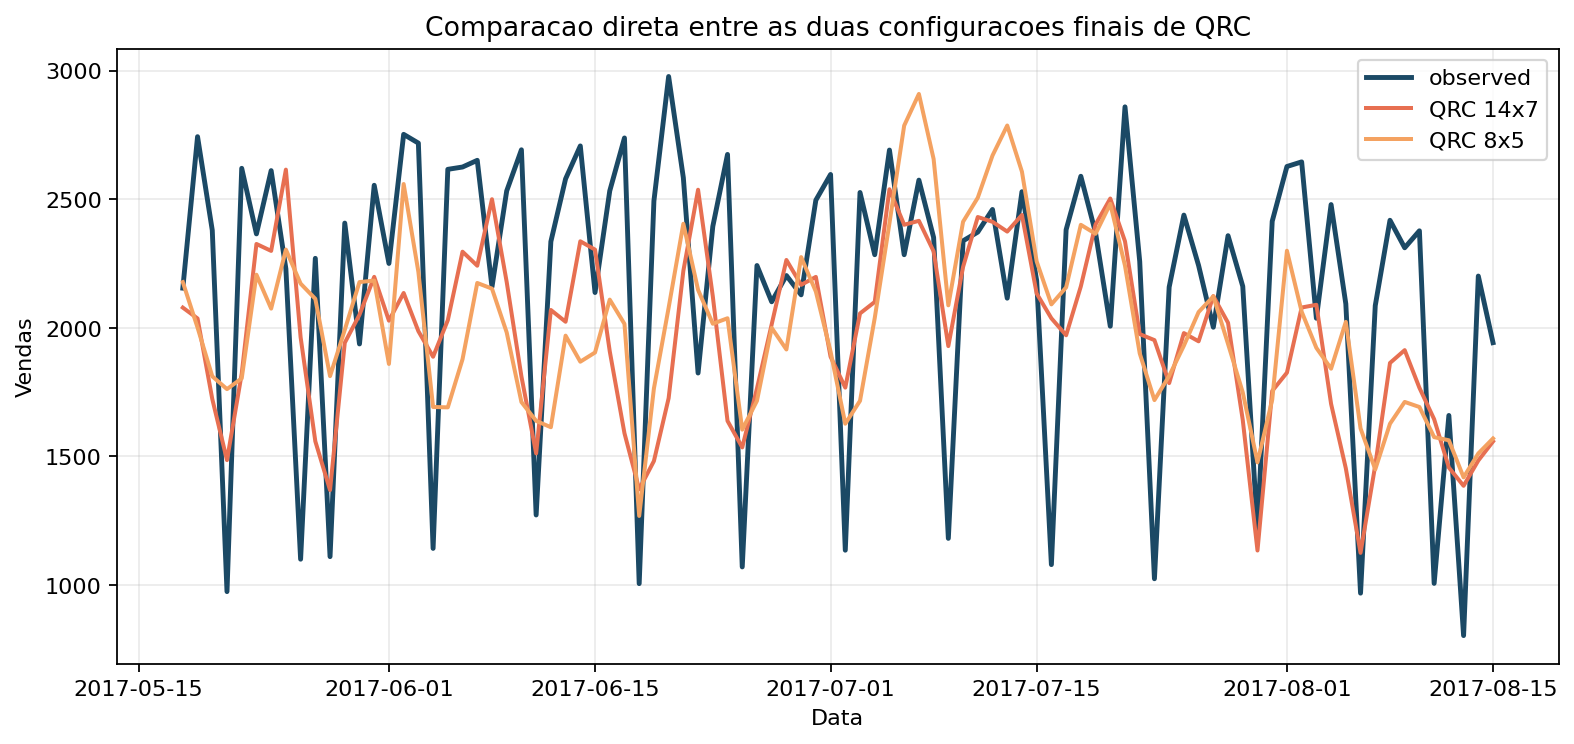
\includegraphics[keepaspectratio,alt={Comparacao direta entre as configuracoes QRC14x7 e QRC8x5.}]{computational_results_20260402_222902/qrc_14x7_vs_8x5.png}}

\pandocbounded{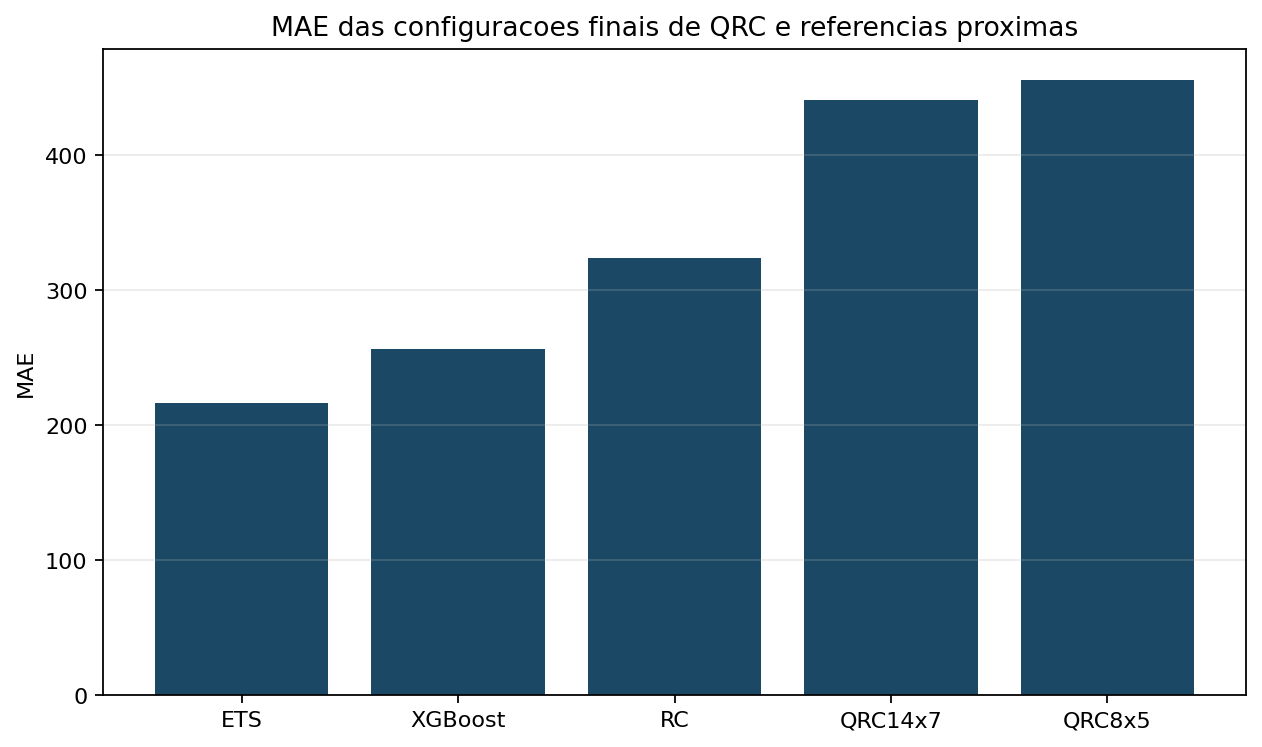
\includegraphics[keepaspectratio,alt={Comparacao em barras para o MAE entre modelos de referencia e QRC.}]{computational_results_20260402_222902/qrc_focus_mae_bars.png}}

A leitura dos dois pontos e clara:

\begin{itemize}
\tightlist
\item
  \texttt{14x7} foi melhor que \texttt{8x5} nas quatro metricas no run direto;
\item
  \texttt{8x5} permaneceu relevante porque sua funcao objetivo penalizada era melhor;
\item
  o trade-off entre desempenho e complexidade foi real, nao artificial.
\end{itemize}

\subsection{7. Comparacao com RC e tecnicas classicas}\label{7-comparacao-com-rc-e-tecnicas-classicas}

O QRC precisa ser lido ao lado do benchmark herdado, nao isoladamente.

\begin{longtable}[]{@{}lllll@{}}
\toprule\noalign{}
Modelo & MAE & RMSE & WAPE & sMAPE \\
\midrule\noalign{}
\endhead
\bottomrule\noalign{}
\endlastfoot
ETS & 216.303 & 307.638 & 0.0999 & 0.1042 \\
XGBoost & 256.666 & 332.828 & 0.1185 & 0.1237 \\
RC & 324.294 & 423.417 & 0.1498 & 0.1653 \\
QRC14x7 & 441.286 & 525.325 & 0.2038 & 0.2269 \\
QRC8x5 & 455.833 & 526.949 & 0.2105 & 0.2342 \\
\end{longtable}

O ponto central do estudo e este:

\begin{itemize}
\tightlist
\item
  \texttt{QRC14x7} ficou cerca de 36.1\% acima do \texttt{RC} em \texttt{MAE};
\item
  \texttt{QRC14x7} ficou cerca de 104.0\% acima do \texttt{ETS} em \texttt{MAE};
\item
  ainda assim, o pipeline quantico funcionou de ponta a ponta no mesmo recorte de negocio.
\end{itemize}

\subsection{8. O que os resultados mostram e o que eles nao mostram}\label{8-o-que-os-resultados-mostram-e-o-que-eles-nao-mostram}

\subsubsection{8.1 O que mostram}\label{81-o-que-mostram}

\begin{itemize}
\tightlist
\item
  QRC pode ser implementado de modo didatico e reprodutivel com Qiskit;
\item
  tuning de \texttt{qubits} e \texttt{window} importa muito;
\item
  o melhor QRC do projeto foi \texttt{14x7};
\item
  comparacoes honestas sao possiveis no mesmo recorte do Favorita.
\end{itemize}

\subsubsection{8.2 O que nao mostram}\label{82-o-que-nao-mostram}

\begin{itemize}
\tightlist
\item
  que QRC seja superior a tecnicas classicas neste problema;
\item
  que aumentar qubits sempre melhora desempenho;
\item
  que o estudo atual esgote o espaco de arquiteturas quanticas possiveis.
\end{itemize}

\subsection{9. A contribuicao didatica do estudo final}\label{9-a-contribuicao-didatica-do-estudo-final}

O estudo final nao vale apenas pela tabela de metricas. Ele vale porque fecha uma trilha de ensino completa:

\begin{enumerate}
\def\labelenumi{\arabic{enumi}.}
\tightlist
\item
  do problema de negocio;
\item
  aos baselines;
\item
  ao RC classico;
\item
  ao tuning;
\item
  ao benchmark justo;
\item
  a ponte quantica;
\item
  ao QRC implementado e comparado.
\end{enumerate}

Essa sequencia e o que transforma o conjunto dos sete artigos em um material "101" real para QRC.

\subsection{10. O que o leitor aprendeu do artigo 1 ao 7}\label{10-o-que-o-leitor-aprendeu-do-artigo-1-ao-7}

Ao final da serie, o leitor passou a saber:

\begin{itemize}
\tightlist
\item
  formular um problema real de previsao de demanda;
\item
  construir um protocolo temporal correto;
\item
  comparar baselines, IA classica, RC e QRC;
\item
  ler e modificar as implementacoes do projeto;
\item
  interpretar resultados negativos ou medianos sem perder valor cientifico;
\item
  entender QRC como extensao do paradigma de reservatorio, e nao como curiosidade isolada.
\end{itemize}

\subsection{11. Conclusao}\label{11-conclusao}

O QRC do projeto funciona, ensina, compara e fecha a serie de forma honesta. O melhor resultado puro ficou em \texttt{14x7}; o melhor compromisso com penalizacao de complexidade ficou em \texttt{8x5}. Nenhum dos dois venceu os melhores modelos classicos no recorte do Favorita, mas ambos cumprem o papel mais importante desta obra: ensinar, de forma continua e reproduzivel, como sair do zero e chegar a um estudo completo de Quantum Reservoir Computing aplicado a um problema real.

\subsection{Entregaveis associados no repositorio}\label{entregaveis-associados-no-repositorio}

\begin{itemize}
\tightlist
\item
  implementacao do QRC: \texttt{code/qrc/}
\item
  tuning e funcao objetivo: \texttt{code/qrc/objective.py}, \texttt{code/qrc/OBJECTIVE.md}
\item
  benchmark consolidado: \texttt{code/RESULTS.md}
\item
  artefatos deste artigo: \texttt{computational\_results\_20260402\_222902/}
\end{itemize}

\subsection{Referencias}\label{referencias}

\begin{itemize}
\tightlist
\item
  Fujii, K.; Nakajima, K. Harnessing disordered-ensemble quantum dynamics for machine learning.
\item
  Ghosh, S. et al. Quantum reservoir processing.
\item
  Qiskit documentation.
\item
  Jaeger, H. The "echo state" approach to analysing and training recurrent neural networks.
\item
  Monzani, F.; Ricci, E.; Nigro, L.; Prati, E. QRC-Lab: An Educational Toolbox for Quantum Reservoir Computing. arXiv:2602.03522.
\end{itemize}

        \end{document}
